\chapter{Data Samples and Event Selection~~~~[DONE]}\label{ch:data}
The data used in this analysis were collected in late 2017 by the CMS Experiment during Run II of the LHC. At this time, the LHC delivered two sets of \pp collisions, at \serag (2017G) and at \serah (2017H). This chapter details the information related to data collection and Monte Carlo simulations associated with these data taking periods. Additionally, details regarding the object identification criteria and event selection are provided.

%%%%%%%%%%%%%%%%%%%%%%%%%%%%%%%%%%%%%%
%%%     Dataset 
%%%%%%%%%%%%%%%%%%%%%%%%%%%%%%%%%%%%%%


\section{Datasets}\label{ch:data:dataset}
Data used in this thesis are from the LHC run eras 2017G and 2017H, consisting of \pp collisions at \serag and \serah, respectively. [Add LUMI] Names of the data streams and relevant run era and reconstruction version identifications are listed in Table~\ref{tab:dataset13} and Table~\ref{tab:dataset5}. 
%%%% 5 TeV datastreams
\begin{table}[htbp]
\begin{center}
\scalebox{1.0}{
\begin{tabular}{l l}
\hline {Data stream} &  {Run \& version}  \\
\hline \hline
SingleMuon      &       Run2017G-17Nov2017-v1   \\
HighEGJet       &       Run2017G-17Nov2017-v2          \\
\hline
\end{tabular}}
\end{center}

\caption{Data streams and the respective run and reconstruction versions for the 2017G (5.02 \TeV) data taking.}
\label{tab:dataset5}
\end{table}

%%%% 13 TeV datastreams
\begin{table}[htbp]
\begin{center}
\scalebox{1.0}{
\begin{tabular}{l l}
\hline {Data stream} &  {Run \& version}  \\
\hline \hline
SingleMuon      &       Run2017H-17Nov2017-v2   \\
HighEGJet       &       Run2017H-17Nov2017-v1          \\
\hline

\end{tabular}}
\end{center}

\caption{Data streams and the respective run and reconstruction versions for the 2017H (13 \TeV) data taking.}
\label{tab:dataset13}
\end{table}



\section{Triggers}\label{ch:data:triggers}
All events considered must have at least one lepton selected by the relevant trigger path. For muons, the kinematic requirement is $\pt>17\GeV$ and $|\eta|<2.4$ for both \serag and \serah. For electrons, the kinematic requirement is $\pt>20\GeV$ ($\pt>17\GeV$) and $|\eta|<2.5$ for \serag (\serah). Additional isolation and reconstruction quality criteria, which are less restrictive than the offline selection criteria, are applied at the trigger level. Names of the trigger paths are listed in  Table~\ref{tab:triggers}

%%%% triggers
\begin{table}[htbp]
\begin{center}
\begin{tabular}{c c}
\hline
\serah    & \serag  \\
\hline \hline
\verb|HLT_HIEle20_WPLoose_Gsf|  & \verb|HLT_HIEle17_WPLoose_Gsf| \\
\hline
\verb|HLT_HIMu17|   &  \verb|HLT_HIMu17| \\
\hline
\end{tabular}
\end{center}
\caption{Data streams and reconstruction versions for the 2017G (5.02 \TeV) data taking.}
\label{tab:triggers}
\end{table}

%%%%%%%%%%%%%%%%%%%%%%%%%%%%%%%%%%%%%%
%%%     Lumi Calibration 
%%%%%%%%%%%%%%%%%%%%%%%%%%%%%%%%%%%%%%

\section{Luminosity}\label{ch:lumi}
Data used for physics analyses are required to pass the quality certification regarding operation of detector subsystems during the data taking period. The list of data taking periods with highest quality requirements are provided in a golden JSON. The JSON files containing the selected data segments for 2017G (\serag) and 2017H (\serah) are: \\
\centerline{\texttt{\small Cert\_306546-306826\_5TeV\_EOY2017ReReco\_Collisions17\_JSON.txt}}
\centerline{\texttt{\small Cert\_306896-307082\_13TeV\_PromptReco\_Collisions17\_JSON\_LowPU\_lowPU.txt}}
%
Pileup conditions during the data taking periods are shown in Figure~\ref{fig:data:lumiPU13}, with an average of $\langle\mu\rangle=3$ collisions per bunch crossing. The instantaneous luminosity per day is shown in Figure~\ref{fig:data:lumiperday5}. Uncertainties on the luminosity measurement are 1.7\% (3.5\%) for the certified data at \serah (\serag). The total integrated luminosity collected by the data streams during \serag and \serah are listed in Table~\ref{tab:lumis}~\cite{LumiPOGNumbers}.
\begin{figure}[htbp]
\centering
  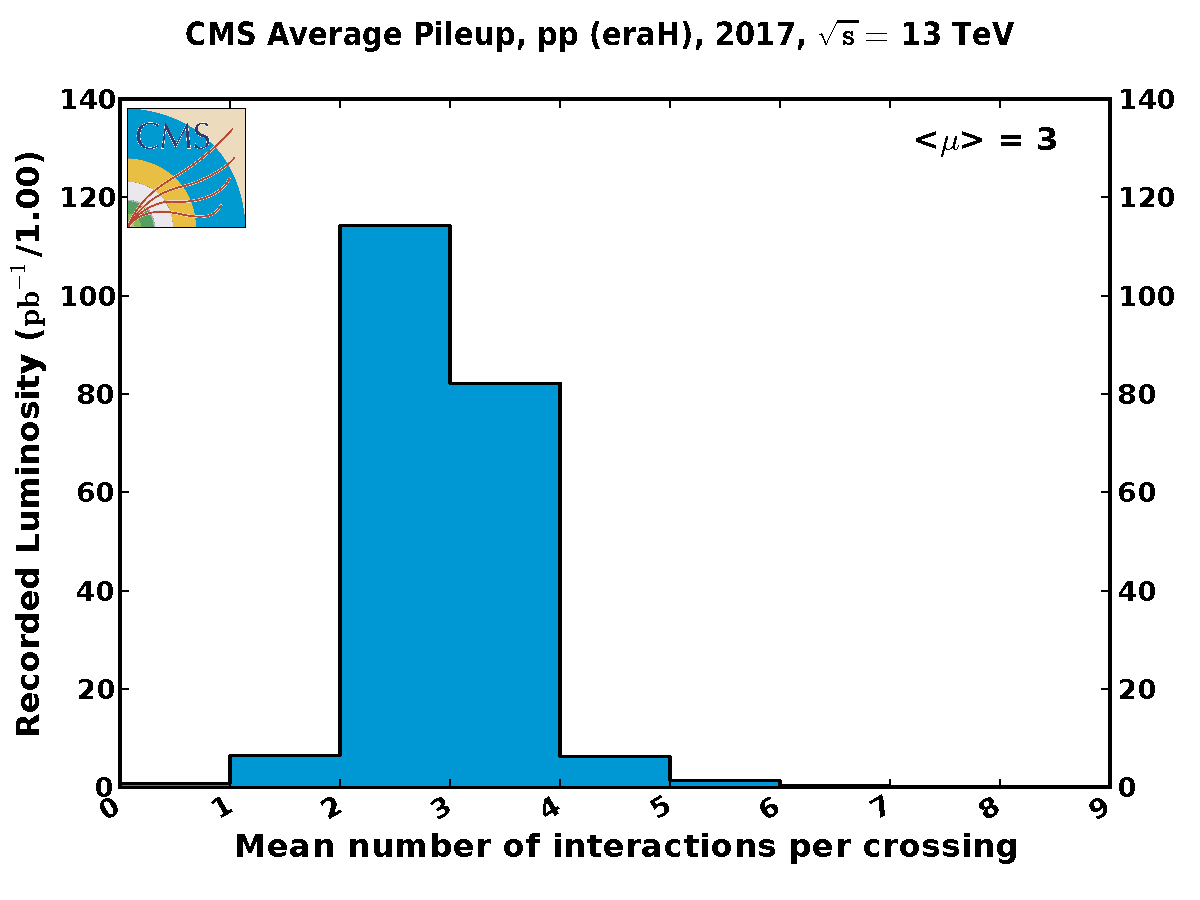
\includegraphics[width=0.75\textwidth]{plots/Data/pileup_pp_lowPU_2017.pdf}
  %https://cds.cern.ch/record/40524
  \caption{Distribution of the number of interactions per bunch crossing for the low pileup \sh (2017H) data taking period. The average number of interactions per crossing is $<\mu> = 3$~\cite{LumiCalibTwiki}.}
  \label{fig:data:lumiPU13}
\end{figure}

\begin{figure}[htbp]
\centering
  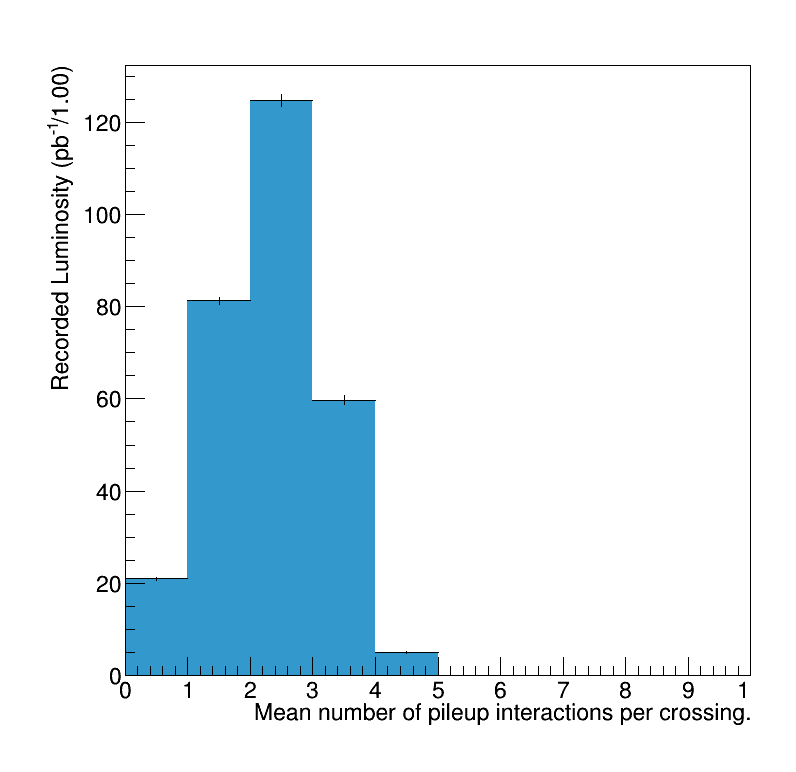
\includegraphics[width=0.75\textwidth]{plots/Data/pileup_5TeV.png}
  %https://cds.cern.ch/record/40524
  \caption{Distribution of the number of interactions per bunch crossing for the \sg (2017G) data taking period. The average number of interactions per crossing is $<\mu> = 2$~\cite{LumiCalibTwiki}.}
  \label{fig:data:lumiPU5}
\end{figure}
\begin{figure}[htbp]
\centering
  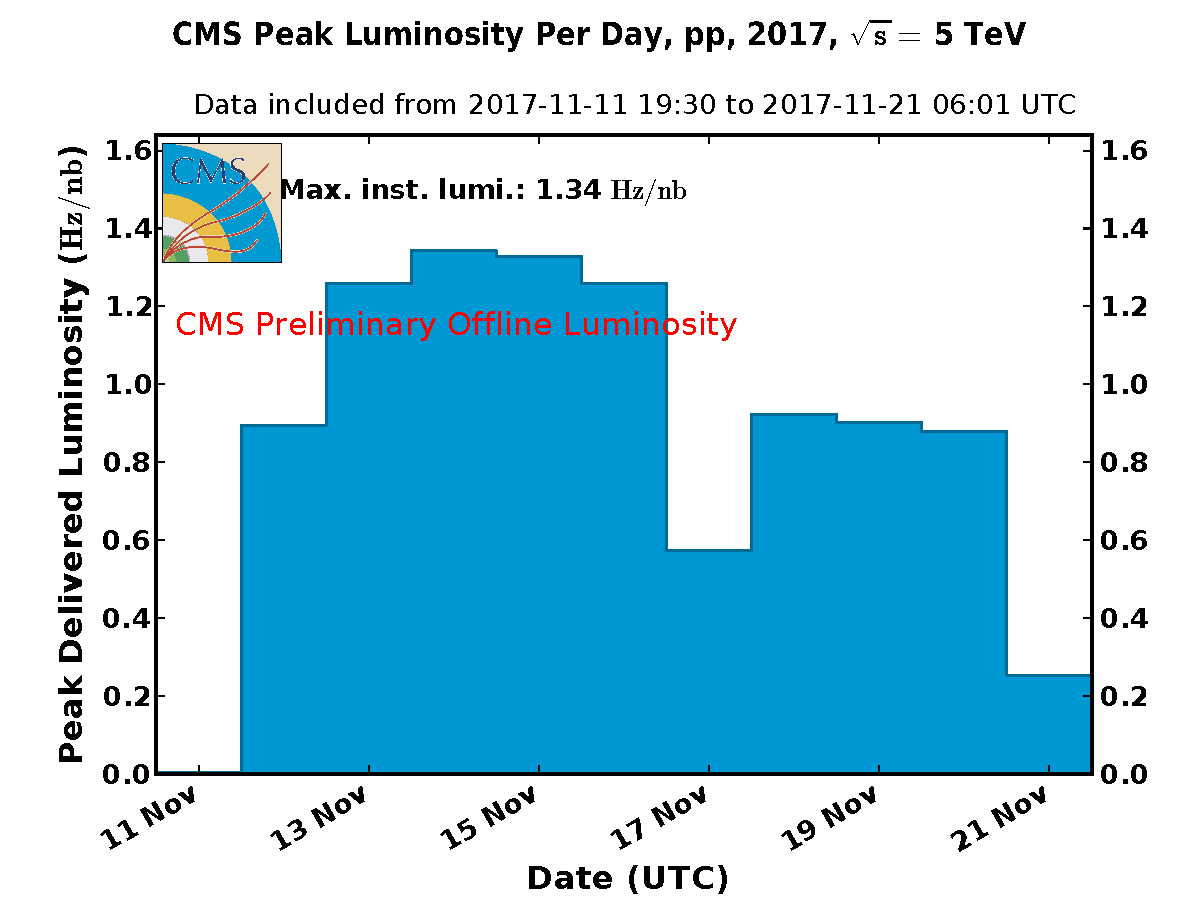
\includegraphics[width=0.6\textwidth]{plots/Data/peak_lumi_per_day_pp_2017_5TeV_NormtagLumi.pdf}
  %https://cds.cern.ch/record/40524
  \caption{Peak instantaneous luminosity per day during the \sg (2017G) data taking period~\cite{LumiCalibTwiki}.}
  \label{fig:data:lumiperday5}
\end{figure}
%%%% lumi values
\begin{table}[htbp]
\begin{center}
\scalebox{1.0}{
\begin{tabular}{c c c}
\hline {\s [\TeV]} & {Run Era} &  {Luminosity [\invpb]}  \\
\hline \hline
5.02  & 2017G    &   $199.2 \pm   3.39$   \\
13    & 2017H    &   $291.1 \pm  11.64$   \\
\hline
\end{tabular}}
\end{center}

\caption{Datasets and their respective integrated luminosity measurements.}
\label{tab:lumis}
\end{table}

%% Is there a specific thing to cite if you use brilcalc to get the lumi out of the trigger path


%%%%%%%%%%%%%%%%%%%%%%%%%%%%%%%%%%%%%%
%%%     Simulated Samples & info 
%%%%%%%%%%%%%%%%%%%%%%%%%%%%%%%%%%%%%%

\section{Simulated samples}\label{ch:data:sim}
Several simulated Monte Carlo (MC) samples are used in the descriptions of signal and background processes. The \Wpm and Z boson signal events are simulated at next-to-leading order (NLO) with up to two outgoing partons at Born level by \MGvATNLO~2.3.3~\cite{Alwall:2014hca}. An additional set of simulations of the \Wpm and Z signal processes are provided at NLO by \POWHEG~2.0~\cite{Alioli:2008gx,Frixione:2007vw,powheg:2010,Alioli:2010xd} for the \Wpm and \MINLO~\cite{Hamilton:2012rf} for the Z. Background samples (di-boson and \ttbar) are also simulated with \POWHEG~2.0. Underlying event modeling, parton showering, hadronization, and final state radiation are done by \PYTHIA~8.230~\cite{Sjostrand:2014zea}, using tune CP5~\cite{Sirunyan:2019dfx} and default parton distribution functions (PDFs) provided by NNPDF3.1~\cite{Ball:2017nwa}. Primary sample names and their respective production cross sections are listed in Table~\ref{tab:allSamples5} (Table~\ref{tab:allSamples13}) for \serag (\serah).

The MC samples also include simulation of additional events occurring in the same and adjacent bunch crossings (pileup). The distribution of pileup interactions is simulated to match the corresponding conditions in data. For all MC, simulation of detector response is performed by \GEANTfour~\cite{Agostinelli:2002hh}, with full event reconstruction being done using the same algorithms used to reconstruct data. Object and event reconstruction was described in Chapter~\ref{ch:reco}. 

%%% 5 TeV MCs
\begin{table}[htbp]
\begin{center}
\scalebox{0.9}{
\begin{tabular}{llr}
\hline
{Sample name} & {Generator} &{~~~Cross section~[pb]} \\
\hline \hline
W+Jets & \aMCATNLO & 21159 \\
\hline
$WW\to 2\ell 2\nu$  & \POWHEG & 2.52 \\
$WZ\to 3\ell \nu$  & \POWHEG & 1.23 \\
$ZZ\to 4\ell$  & \POWHEG & 2.75 \\
$ZZ\to 2\ell 2\nu$  & \POWHEG & 2.75 \\
\hline
\ttbar  & \POWHEG &  69.5 \\
\hline
DY+jets$\to\ell\ell$ ~~~ & \aMCATNLO & 2141  \\
\hline
\end{tabular}}
\end{center}
\caption{Names and cross sections of simulated samples corresponding to run era 2017G (\serag).}
\label{tab:allSamples5}
\end{table}


%%% 13 TeV MCs
\begin{table}[htbp]
\begin{center}
\scalebox{0.9}{
\begin{tabular}{llr}
\hline
{Sample name}  & {Generator}& {~~~Cross section~[pb]} \\
\hline \hline
$W$+0 jets & \aMCATNLO & 49397\\
$W$+1 jets  &\aMCATNLO & 8087 \\
$W$+2 jets  & \aMCATNLO & 3176 \\
\hline
ZZ  & \POWHEG  & 16.523 \\
$WZ\to 3\ell\nu$  & \POWHEG  & 4.912 \\
$WZ\to 2\ell 2\nu$  & \POWHEG  & 12.6 \\
\hline
$\ttbar \to 2\ell 2\nu$  & \POWHEG  & 88.29 \\
$\ttbar \to \mathrm{semileptonic}$ ~~~ & \POWHEG  & 365.35 \\
$\ttbar \to \mathrm{hadronic}$  & \POWHEG  & 377.96 \\
\hline
DY+jets$\to\ell\ell$  & \aMCATNLO & 6225.42 \\
\hline
\end{tabular}}
\end{center}
\caption{Names and cross sections of simulated samples corresponding to run era 2017H (\serah).}
\label{tab:allSamples13}
\end{table}



% %%% 5 TeV MCs
% \begin{table}[htbp]
% \begin{center}
% \scalebox{0.9}{
% \begin{tabular}{lrr}
% \hline
% {Sample name} & {Cross section~[pb]} \\
% \hline \hline
% WJetsToLNu\_TuneCP5\_5020GeV-amcatnloFXFX-pythia8 & 21159 \\
% \hline
% WWTo2L2Nu\_NNPDF31\_TuneCP5\_5p02TeV-powheg-pythia8 & 2.52 \\
% WZTo3LNU\_NNPDF30\_TuneCP5\_5p20TeV-powheg & 1.23 \\
% ZZTo4L\_5p02TeV\_powheg\_pythia8 & 2.75 \\
% ZZTo2L2Nu\_5p02TeV\_powheg\_pythia8 & 2.75 \\
% \hline
% TT\_TuneCP5\_5p02TeV-powheg-pythia8 &  69.5 \\
% \hline
% DYJetsToLL\_MLL-50\_TuneCP5\_5020GeV-amcatnloFXFX-pythia8 & 2141  \\
% \hline
% \end{tabular}}
% \end{center}
% \caption{Names and cross sections of simulated samples corresponding to run era 2017G (5.02 TeV).}
% \label{tab:allSamples5}
% \end{table}


% %%% 13 TeV MCs
% \begin{table}[htbp]
% \begin{center}
% \scalebox{0.9}{
% \begin{tabular}{lrr}
% \hline
% {Sample name} & {Cross section~[pb]} \\
% \hline \hline
% WJetsToLNu\_0J\_TuneCP5\_13TeV-amcatnloFXFX-pythia8 & 49397\\
% WJetsToLNu\_1J\_TuneCP5\_13TeV-amcatnloFXFX-pythia8 & 8087 \\
% WJetsToLNu\_2J\_TuneCP5\_13TeV-amcatnloFXFX-pythia8 & 3176 \\
% \hline
% ZZ\_TuneCP5\_13TeV-pythia8  & 16.523 \\
% WZTo3LNu\_TuneCP5\_13TeV-powheg-pythia8  & 4.912 \\
% WWTo2L2Nu\_TuneCP5\_13TeV-powheg-pythia8  & 12.6 \\
% \hline
% TTTo2L2Nu\_TuneCP5\_13TeV-powheg-pythia8  & 88.29 \\
% TTToSemiLeptonic\_TuneCP5\_13TeV-powheg-pythia8  & 365.35 \\
% TTToHadronic\_TuneCP5\_13TeV-powheg-pythia8  & 377.96 \\
% \hline
% DYJetsToLL\_M-50\_TuneCP5\_13TeV-amcatnloFXFX-pythia8 & 6225.42 \\
% \hline
% \end{tabular}}
% \end{center}
% \caption{Names and cross sections of simulated samples corresponding to run era 2017H (13 TeV).}
% \label{tab:allSamples13}
% \end{table}




% %%%%%%%%%%%%%%%%%%%%%%%%%%%%%%%%%%%%%%
% %%%     Signal & Bkg modeling
% %%%%%%%%%%%%%%%%%%%%%%%%%%%%%%%%%%%%%%
% \section{Modeling of Signal and Background}\label{ch:data:modelSigAndBkg}
% %% Discuss the signal and background MC here
% Monte Carlo samples are used to model the signal and some of the background processes. The rest of the background is modeled from a data-driven approach. Background processes which are considered are those coming from \ttbar~production, QCD multi-jet production, and  other electroweak processes. 

% \begin{itemize}
% \item \ttbar: top quark pairs produced, with the lepton(s) from the decay products being reconstructed within the fiducial region
% \item Di-Boson production: Cross section predictions are only for the production of a single boson. Di-boson processes $WW$, $WZ$, and $ZZ$ can produce single- or di-lepton signatures satisfying the W or Z selection criteria
% \item \ztt~(\Z background to the \Z): Single \Z production with the \Z decaying to a pair of $\tau$, and the leptons from the $\tau$ decays are reconstruted as \zee~ or \zmm.
% \item \ztt, \zmm, \zee~ (\Z background to the \W): \zll, with one reconstructed lepton in the fiducial region. One of the largest EWK backgrounds to the W.
% \item \wtau: Single W production, where the W decays via a $\tau$ to a $\mu$ or $e$. 
% \item QCD multi-jet events: jets faking isolated leptons
% \item High \pt photon: conversion into an electron of a hard photon from the process $pp\rightarrow\gamma+\mathrm{jets}$. Affects only the electron channel.
% \end{itemize}

% The QCD background is the most significant background for the W measurement, with a larger impact in the electron channel than the muon channel due to the additional contribution of the $\gamma+\mathrm{jets}$ photon conversions into electrons. In addition, the \wtau~ and \ztt~ backgrounds become significant at higher \met. 

% Signal samples for both W and Z production are generated with aMC@NLO interface to Pythia8 for parton showering, using the CP5 tune. Alternative samples containing event generation by POWHEG and minlo and shower modeling by PHOTOS are used for cross-checks and evaluation of uncertainties. Background samples for top production and diboson production are generated with POWHEG intefaced to Pythia8 using the CP5 tune. 




%%%%%%%%%%%%%%%%%%%%%%%%%%%%%%%%%%%%%%
%%%     Event Selection
%%%%%%%%%%%%%%%%%%%%%%%%%%%%%%%%%%%%%%
\section{Event Selection \& Fiducial Region}
 \subsubsection{Reconstructed Event Selection}
Preliminary \Wpm and \Z event candidates are identified by the presence of at least one lepton identified by the single electron and single muon triggers described in Section~\ref{ch:data:triggers}. These are further selected by applying the offline electron or muon reconstruction identification criteria described in Section~\ref{ch:IdIso}. 
A \Z boson event requires the presence a pair of oppositely charged leptons ($e^{+}e^{-}$ or $\mu^{+}\mu^{-}$), each of the charged leptons being identified by the trigger, each of the charged leptons fulfilling the ID requirements in Section~\ref{ch:IdIso}, and an invariant mass of \masswindow. 
Selection of a \Wpm candidate requires one charged lepton identified by the trigger and passing all ID requirements in Section~\ref{ch:IdIso}. A veto is applied to events containing additional same-flavor leptons passing a loose identification requirement. Additionally, \Wpm events are required to have an invariant mass $\mt > 40\GeV$, with \mt defined by: 
$\mt = \sqrt{ 2 \pt \met ( 1 - \cos(\Delta\phi) ) }$, where $\Delta\phi$ is the angle between the lepton and \vmet in the transverse plane.

\subsubsection{Fiducial Region}
The fiducial region for the \Wpm and \Z acceptance at generator-level emulates the selection at reconstruction level. This requires kinematic cuts $\pt > 25 \GeV$ and $|\eta| < 2.4$ for all charged leptons. Additionally, the \Z boson fiducial region includes a requirement on the dilepton mass: \masswindow. The fiducial region for the \Wpm includes the transverse mass requirement $\mt>40\GeV$.


%%%%%%%%%%%%%%%%%%%%%%%%%%%%%%%%%%%%%%
%%%     object definition
%%%%%%%%%%%%%%%%%%%%%%%%%%%%%%%%%%%%%%
\section{Object Identification}\label{ch:IdIso}
The \Wpm (\Z) boson candidates are identified by the presence of one (two) well-identified leptons passing a strong set of criteria ensuring proper reconstruction and identification. This section contains a description of the identification requirements for the \wlnu and \zll signal leptons, as well as the requirements for the lepton veto for the \Wpm selection.

\subsection{Electrons}\label{ch:IdIso:Ele}
Electrons originating from a candidate \Wpm or \Z are required to pass the standard cut-based identification with medium working point. The thresholds for observables required to pass this requirement are listed in Table~\ref{tab:Data:Sel:Ele}~\cite{EgammaIDIsoCuts}. The \Wpm selection requires the absence of additional electrons in the event. The veto is performed using additional electrons fulfilling the loose working point identification requirements, with criteria listed in Table~\ref{tab:Data:Sel:EleVeto}. 

\begin{itemize}
    \item $\pt > 25 \GeV$: high-\pt leptons
    \item $|\eta|< 2.4$: make the electron fiducial region match the muon fiducial region
    \item ($\Delta\eta_{In}$,$\Delta\phi_{In}$): ECAL supercluster and track are matched when extrapolating to vertex
    \item $\sigma_{i\eta i\eta}$: electron-like cluster profile
    \item H/E: Allow only a small amount of activity in the HCAL in the region behind the ECAL electron
    \item $|d_{0,bs}|$,~$|d_{z,bs}|$: small impact parameters in the transverse plane and longitudinal axis, relative to the beam spot
    \item $|1/E-1/p|$: 
    \item $\mathrm{Iso_{PF}}/\pt$: isolated leptons less likely to be from a jet
    \item Missing Hits: Require very few missing hits in tracker layers
    \item Conversion fit veto probability should be < $10^{-6}$, electron unlikely to be from $\gamma$ conversion
\end{itemize}


%%%% Table containing the Ele ID+Iso cuts
\begin{table}[htbp]
\begin{center}
\scalebox{0.8}{
\begin{tabular}{|c|c|c|}
\hline
Observable & Barrel & Endcap \\
\hline \hline
$p_T$ & \multicolumn{2}{c|}{$> 25$ \GeV} \\ \hline % OK
$|\eta|$ & \multicolumn{2}{c|}{$< 2.4$}\\ \hline% OK
$\Delta\eta_{In}$ & $< 0.0032$ & $< 0.00632$\\ \hline% OK
$\Delta\phi_{In}$ & $< 0.0547$ & $< 0.0394$\\ \hline% OK
$\sigma_{i\eta i\eta}$ & $<  0.0106$ & $< 0.0387$\\ \hline% OK
H/E & $< 0.046+1.16/E_{SC}+0.0324\rho/E_{SC}$ & $< 0.0275+2.52/E_{SC}+0.183\rho/E_{SC}$\\ \hline%
$|d_{0,bs}|$ & $< 0.05$ & $< 0.10$\\ \hline% OK
$|d_{z,bs}|$ & $< 0.10$ & $< 0.20$\\ \hline% OK
$|1/E-1/p|$ & $< 0.184$& $< 0.0721$\\ \hline% OK
$\mathrm{Iso_{PF}}/$\pt &$< 0.0478+0.506/p_{\mathrm{T},ele}$ &$< 0.0658+0.963/p_{\mathrm{T},ele}$ \\ \hline
Missing Hits & \multicolumn{2}{c|}{$\leq 1$}\\ \hline
\multicolumn{3}{|c|}{Pass conversion veto}\\
\hline
\end{tabular} }
\end{center}
\caption{Reconstructed identification and isolation criteria fulfilling the medium cut-based ID for electron selection.}
\label{tab:Data:Sel:Ele}
\end{table}

%% Table containing the Electron ID+Iso Veto cuts
%% Cut Type
\begin{table}[htbp]
\begin{center}
\scalebox{0.8}{
\begin{tabular}{|c|c|c|} %%%% Table needs vertical lines
\hline
Observable & Barrel & Endcap \\
\hline \hline
$p_T$ & \multicolumn{2}{c|}{$> 25$ \GeV} \\ \hline % OK
$|\eta|$ & \multicolumn{2}{c|}{$< 2.4$}\\ \hline% OK
$\Delta\eta_{In}$ & $< 0.00463$ & $< 0.00814$\\ \hline
$\Delta\phi_{In}$ & $< 0.148$ & $< 0.19$\\ \hline
$\sigma_{i\eta i\eta}$ & $< 0.0126$ & $< 0.0457$\\ \hline
H/E & $< 0.05+1.16/E_{SC}+0.0324\rho/E_{SC}$ & $< 0.05+2.54/E_{SC}+0.183\rho/E_{SC}$\\ \hline%
$|d_{0,bs}|$ & $< 0.05$ & $< 0.10$\\ \hline
$|d_{z,bs}|$ & $< 0.10$ & $< 0.20$\\ \hline
$|1/E-1/p|$ & $<0.209$& $< 0.132$\\ \hline
$\mathrm{Iso_{PF}}/$\pt &$< 0.198+0.506/p_{T,ele}$ &$< 0.203+0.963/p_{T,ele}$ \\ \hline
Missing Hits & $\leq 2$ & $\leq 3$\\ \hline
\multicolumn{3}{|c|}{Pass conversion veto}\\
\hline
\end{tabular}}
\end{center}
\caption{Reconstructed identification and isolation criteria fulfilling the loose cut-based ID for electron selection used as a veto on \Wpm events with additional leptons present.}
\label{tab:Data:Sel:EleVeto}
\end{table}

\subsection{Muons}\label{ch:IdIso:Mu}
Muons originating from a candidate \Wpm or \Z are required to pass the standard cut-based identification with tight working point with tight working point requirement on the muon PF isolation. The thresholds for observables required to pass this requirement are listed in Table~\ref{tab:Data:Sel:Mu}~\cite{MuonIDIsoCuts}. As in the electron channel, the \Wpm selection requires the absence of additional muons in the event. The veto is performed using additional muons fulfilling the loose working point identification requirements and no isolation requirement, with criteria listed in Table~\ref{tab:Data:Sel:Mu:Veto}. 
\begin{itemize}
    \item $\pt > 25 \GeV$: high-\pt leptons only
    \item $|\eta| < 2.4$: muons within the appropriate detector volume
    \item Muons must be identified as such by particle flow muon ID and be reconstructed by the GlobalMuon algorithm
    \item $\chi^2/$ndof: Quality of the global muon fit must satisfy $\chi^2/$ndof < 10
    \item \# Valid Mu Hits: At least one good muon system hit is required in the GlobalMuon fit
    \item \# Matched Stations: Muon stations have at least 2 muon segments
    \item \# Tracker Layers: At least 6 tracker layers should have hits
    \item \# Valid Pixel Hits: at least one hit in the pixel tracker associated with the muon
    \item $|d_{0,bs}|$,~$|d_{z,bs}|$: loose cut on impact parameters in the transverse plane and longitudinal axis, relative to the beam spot 
    \item $\mathrm{Iso_{PF}}/\pt$: Muons must be isolated. Similar to electrons, the particle-flow isolation is used. 
\end{itemize}


%%%% Table containing the Ele ID+Iso cuts
\begin{table}[htbp]
\begin{center}
\scalebox{0.8}{
\begin{tabular}{|c|c|}
\hline
Observable & Value/Range \\
\hline \hline
\pt & > 25 GeV \\ \hline % OK
$|\eta|$ & $< 2.4$\\ \hline% OK
ID & ~GlobalMuon~ \\ \hline% OK
ID & ~PFMuon~\\ \hline% OK
$\chi^2/$ndof & $< 10$\\ \hline% OK
~\# Valid Mu Hits ~ & $\geq 1$\\ \hline%
~\# Matched Stations ~& $\geq 2$\\ \hline%
~\# Tracker Layers ~& $\geq 6$\\ \hline%
~\# Valid Pixel Hits~ & $\geq 1$\\ \hline%
$|d_{0,bs}|$ & < 0.2 \\ \hline% OK
$|d_{z,bs}|$ & < 0.5 \\ \hline% OK
$\mathrm{Iso_{PF}}/$\pt &$< 0.15$\\
\hline
\end{tabular}}
\end{center}
\caption{Reconstructed identification and isolation criteria fulfilling the cut-based ID with tight isolation requirement for muon selection.}
\label{tab:Data:Sel:Mu}
\end{table}
%%%% Table containing the Ele ID+Iso cuts
\begin{table}[htbp]
\begin{center}
\scalebox{0.8}{
\begin{tabular}{|c|c|c|}
\hline
Observable & Value/Range \\
\hline \hline
\pt & > 10 GeV \\ \hline % OK
$|\eta|$ & < 2.4\\ \hline% OK
ID & \textsc{GlobalMuon} \textbf{OR} \textsc{TrackerMuon}\\ \hline% OK
ID & \textsc{PFMuon}\\ 
\hline
\end{tabular}}
\end{center}
\caption{Reconstructed identification and isolation criteria for identifying additional muons used as a veto on \Wpm boson events.}
\label{tab:Data:Sel:Mu:Veto}
\end{table}

